\section{\textit{Nome do artigo}}


% ============================================================================
\subsection{Referência completa do artigo}

\begin{itemize}
  \item \textbf{Autores:} xxx
  \item \textbf{Local:} xxx
  \item \textbf{\textit{Journal}:} xxx [Qualis XXX]
  \item \textbf{Data:} xxx
  \item \textbf{Referência:} \citeonline{bib:2014:Autor2}
\end{itemize}


% ============================================================================
\subsection{Resumo}
% ..........................................................
\subsubsection{Propósito do artigo}
xxx

% ..........................................................
\subsubsection{Técnicas utilizadas} 
% \begin{itemize}
%   \item xxx
% \end{itemize}  
xxx

% ..........................................................
\subsubsection{Contribuição em relação a artigos anteriores} %mais ou menos 10 linhas
% \begin{itemize}
%   \item xxx
% \end{itemize}  
xxx

% ============================================================================
\subsection{Metodologia}
% Descreva um pouco mais detalhadamente a metodologia e os resultados do artigo. 
% Inclua as figuras que achar mais relevantes.

A Figura \ref{fig:2014:Autor2:figs} mostra as Figuras \ref{fig:2014:Autor2:fig1}
e \ref{fig:2014:Autor2:fig2} agrupadas.

\begin{figure}[ht]
	\centering
	\begin{subfigure}[t]{0.48\textwidth}
		\centering
		
\includegraphics[width=0.70\textwidth]{artigos/2014_Autor2/fig1.png}
		\caption{Figura 1}
		\label{fig:2014:Autor2:fig1}
	\end{subfigure}
 	\begin{subfigure}[t]{0.48\textwidth}
		\centering
		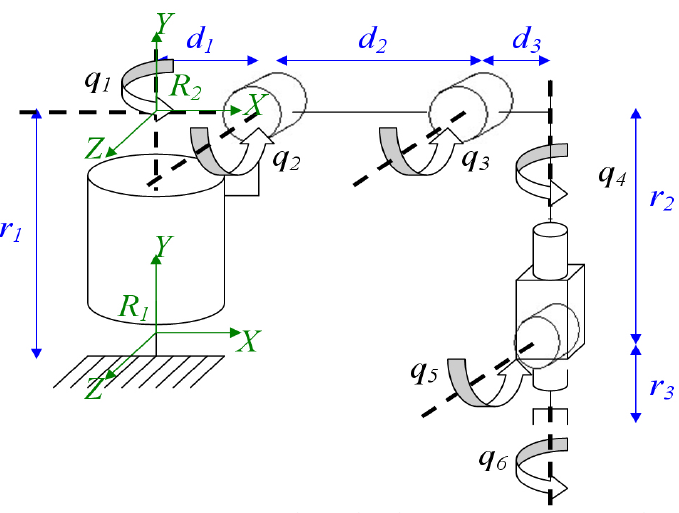
\includegraphics[width=0.70\textwidth]{artigos/2014_Autor2/fig2.png}
		\caption{Figura 2}
		\label{fig:2014:Autor2:fig2}
	\end{subfigure}
	\caption{Agrupamento de figuras.}
	\label{fig:2014:Autor2:figs}
\end{figure}

% ..........................................................
\subsubsection{Resultados}
xxx

% ============================================================================
\subsection{Pontos fortes} %no máximo três
\begin{itemize}
  \item xxx
  \item xxx
  \item xxx
\end{itemize}  

% ============================================================================
\subsection{Limitações} %no máximo três
\begin{itemize}
  \item xxx
  \item xxx
  \item xxx
\end{itemize} 


% ============================================================================
\subsection{Avaliação}
\textbf{(a) Avanço considerável (\textit{Breakthrough}).}
% \textbf{(b) Contribuição significativa.}
% \textbf{(c) Contribuição modesta.}
% \textbf{(d) Contribuição fraca.}
% \textbf{(e) Sem contribuição.}
Justificativa.

% ============================================================================
\subsection{Problema em aberto}
% \begin{itemize}
%   \item xxx
% \end{itemize}  
xxx

% ============================================================================
\subsection{Aspecto obscuro}
% \begin{itemize}
%   \item xxx
% \end{itemize}  
xxx